\subsubsection{Top quark contributions}

\label{EW:top}

\noindent \textbf{Joshua Davies, Kay Schönwald, Matthias Steinhauser, Hantian Zhang~\cite{Davies:2023npk,Davies:2026wbx}.}

\noindent The full top quark contributions, including all sectors of the SM, have been computed analytically in
Refs.~\cite{Davies:2023npk,Davies:2026wbx} in the inverse top quark mass expansion and the high-energy expansion.

In the large-$m_t$ limit~\cite{Davies:2023npk}, expansions up to order $1/m_t^{10}$ have been computed in the Feynman gauge in the limit
\begin{align}
m_t^2 \, \gg \, s, \, |t|, \, m_h^2, \, m_W^2 , \, m_Z^2 \,,
\end{align}
where no additional hierarchy is assumed among the scales on the right-hand side.
%
The calculation has been analytically validated in the general $R_\xi$-gauge by assuming the hierarchy
\begin{align}
    m_t^2 \, \gg \, \xi_W \, m_W^2, \, \xi_Z \, m_Z^2  \, \gg \, s, \, |t|, \, m_h^2, \, m_W^2 , \, m_Z^2 \,,
\end{align}
where $\xi_W, \xi_Z$ are gauge parameters for the $W$ and $Z$ bosons.
%
These parameters appear in combination with gauge boson masses in the gauge boson and Goldstone propagators.
%
It is a valuable and non-trivial analytic validation that $\xi_W$ and $\xi_Z$ drop out in the renormalized amplitudes. 
%
Note that the gauge parameter for the photon, $\xi_\gamma$, drops out after summing all bare two-loop diagrams.
%


In the high-energy limit~\cite{Davies:2026wbx},
the electroweak calculation is much more challenging compared to the QCD case and the large-$m_t$ EW case. In this limit, we perform nested expansions in several small parameters in the following hierarchies in the Feynman gauge:
\begin{align}
    s, \, |t| \,  \gg \, m_t^2, \, m_W^2, \, m_Z^2 \,, (m_h^{\rm int})^2 \, \gg \,  (m_h^{\rm ext})^2\,,
\end{align}
where $m_h^{\rm int}$ denotes the mass of Higgs propagators inside the loop and $m_h^{\rm ext}$ is the mass of the final-state Higgs boson.
%
By identifying these hierarchies, we can first perform an external Higgs mass expansion, followed by expansions in the mass differences among several internal mass parameters as $\delta_X = 1 - m_X/ m_t $ for $ X=W,Z,H$.
Finally and most importantly, we perform a deep high-energy expansion with more than 100 expansion terms around the small-$m_t$ limit.
%
Schematically, the generic structure of the high-energy expansion of the form factors can be written as
\begin{align}
  F &= \sum_{n=-4}^{108} \sum_{i=0}^{2} \sum_{k_W=0}^{{4}}\sum_{k_Z=0}^{{4}}\sum_{k_H=0}^{{4}} 
        c_{ni}^{k_W k_Z k_H}  \: m_t^{n} \:
        (m^{\rm ext}_H)^{2i} \:
        \delta_W^{k_W} \: \delta_Z^{k_Z} \: \delta_H^{k_H} 
        \,,
\end{align}
where $c_{ni}^{k_W k_Z k_H}$ are coefficient functions of $s,t$ and $\log(m_t^2)$, featuring polylogarithmic and elliptic structures.
%
These analytic expressions are numerically evaluated through a Pad\'{e} procedure to increase the radius of convergence of the high-energy expansion across a larger phase space region.
%
The high-energy computation is technically challenging at both the form factor and Feynman integral level, due to drastically increased complexity when the full electroweak sector is taken into account.
%
We have successfully tackled both complexities and achieved a deep high-energy expansion up to the orders $m_t^{108}$, $(m_{H}^{\rm ext})^4$ and $\delta_X^4$. 
We have systematically analysed the convergence properties of our expansion, and we estimate the truncation uncertainty, dominated by the mass-difference expansion, to be about $\pm 1\%$ of the two-loop corrections.
%
For technical details of master integral calculations for the electroweak topologies, we refer to Refs.~\cite{Davies:2025wke,Davies:2022ram,Zhang:2024fcu}.



%%%
The electroweak renormalization follows the standard procedure as outlined in Refs.~\cite{Denner:1991kt,Denner:2019vbn}. 
%
The one-loop form factors are expressed in terms of parameters $\{e,m_W,m_Z,m_t,m_h\}$, and the parameter renormalization is performed with corresponding renormalization constants in the on-shell scheme.
%
The wave functions of the external Higgs bosons are also renormalized in the on-shell scheme.
%
Throughout the entire calculation, all tadpole contributions are consistently included such that all parameter renormalization constants are gauge-parameter independent, while the gauge-parameter dependence only appears in the wave function renormalization constant for the external Higgs boson.
%
This prescription is equivalent to the so-called \textit{Fleischer--Jegerlehner tadpole scheme}~\cite{Fleischer:1980ub}.
%

%%%%
The large-$m_t$ result~\cite{Davies:2023npk} supports the findings of Ref.~\cite{Muhlleitner:2022ijf},
where the top Yukawa-induced effects have been studied, namely that the electroweak corrections near the Higgs boson pair production threshold can lead to a few tens of percent effects with respect to the leading order contribution.
%
This interesting phenomenon is due to the fact that the electroweak corrections lift the destructive interference near the production threshold, where the matrix element is suppressed by the cancellation between triangle and box form factors at leading order.
Similarly, large top Yukawa-induced corrections near the production threshold have been found in Ref.~\cite{Heinrich:2024dnz}.
%
Although the radius of convergence is
limited, this result also serves as an important benchmark for other calculations. 
For example, it has been compared with Ref.~\cite{Bi:2023bnq} in a large-$m_t$ limit and good agreement was observed.

%
The high-energy result~\cite{Davies:2026wbx} has several interesting features.
In the limiting case of $m_h = 0$ and $m_t \to 0$, the leading high-energy expansion starts at $(m_t^2/s)^0$ at two loops, while it only starts at $(m_t^2/s)^1$ at one loop.
%
At NLO EW in this limit, we observe a quadratic and cubic logarithm ($\alpha \log^2(m_t^2/s)$ and $\alpha \log^3(m_t^2/s)$) as the leading logarithmic contribution for the box contributions in form factors $F_1$ and $F_2$, respectively. Note that the triangle contributions are suppressed at high energies due to the $s$-channel Higgs propagator.
%
In Fig.~\ref{fig::rEW_HE}, we present our result in terms of a ``partonic $K$-factor'' $r_{EW} = \frac{\alpha}{\pi} \big( \, \mathcal{U}^{(0,1)} / \mathcal{U}^{(0)} \big)$ up to $\sqrt{s} = 10$~TeV, where we assume the perturbative NLO QCD and EW expansion as $|\mathcal{M}|^2 = \bar{X}_0 \big( \, \mathcal{U}^{(0)} + \frac{\alpha_s}{\pi}\, \mathcal{U}^{(1,0)} + \frac{\alpha}{\pi} \, \mathcal{U}^{(0,1)} \big)$ with an overall prefactor $\bar{X}_0$.
\begin{figure}[t]
\centering
    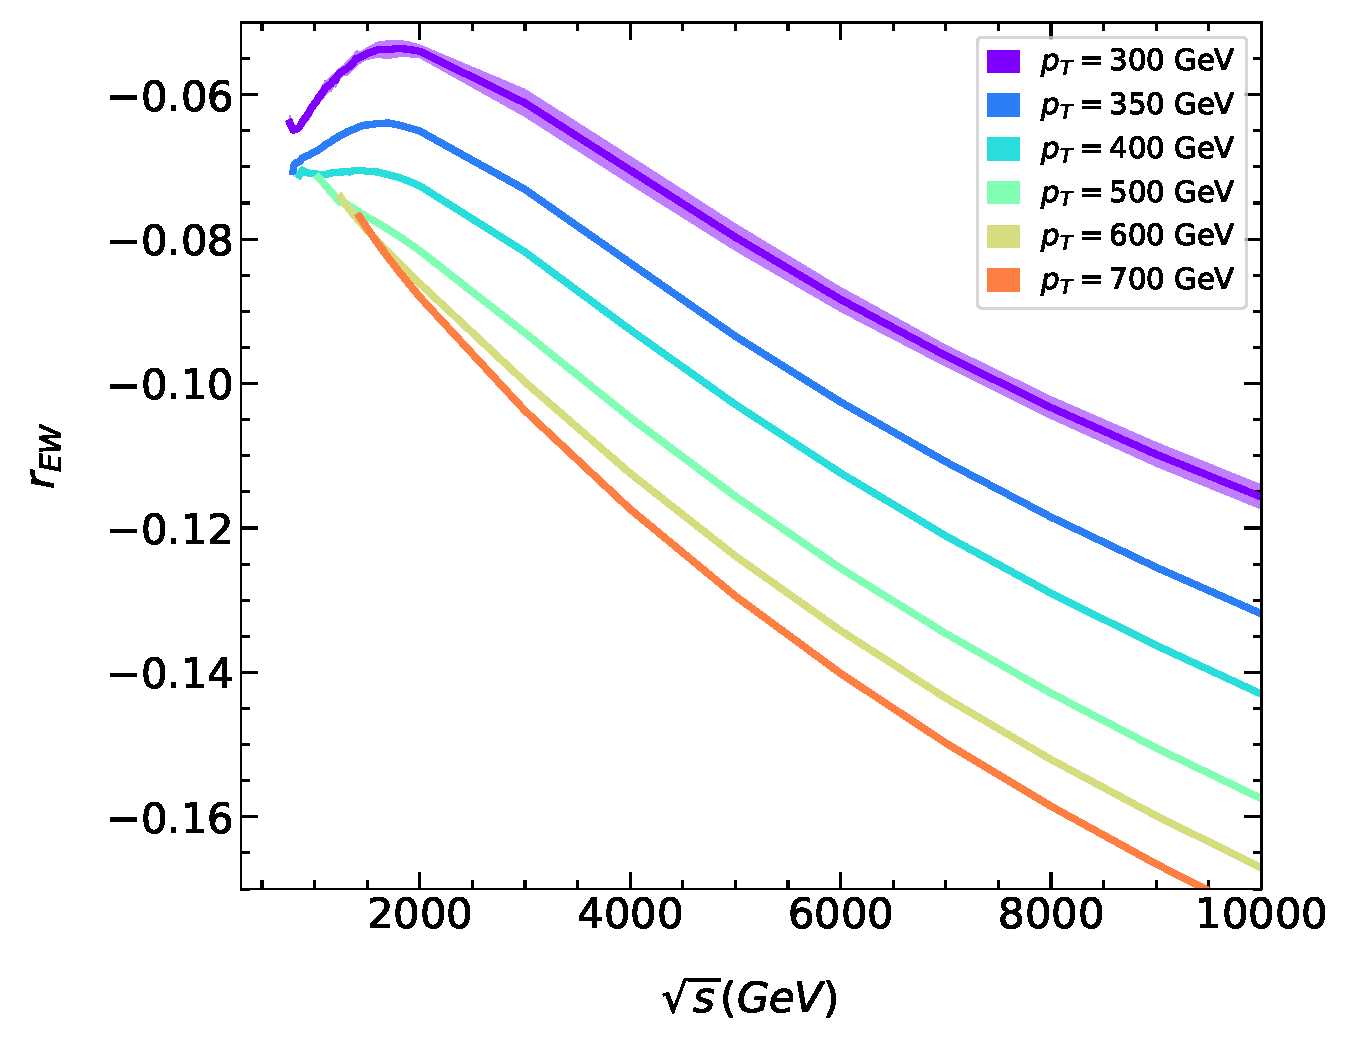
\includegraphics[width=.65\textwidth]{NLO_EW_SM/EW_top/figs/rEW_HE.pdf}
  \caption{\label{fig::rEW_HE}
   $r_{\rm EW}$ for various values of $p_T$ as a function of $\sqrt{s}$.
   The plots show the same data for different ranges of $\sqrt{s}$ on the $x$ axis. The uncertainty band (only visible for $p_T = 300$~GeV) is obtained from the Pad\'{e} approximation, and the truncation uncertainty in the $\delta_X$ and $m_h^{\rm ext}$ expansions is not shown but is estimated to be $\pm1\%$.
   Results shown are from Ref.~\cite{Davies:2026wbx}.
   }
\end{figure}
Our result covers a large phase space ranging from the high-energy limit to fairly low values of Higgs transverse momentum $p_T \gtrsim 350$~GeV.
It shows that these electroweak corrections lead to an effect of order $-10\%$, supporting the observation from Ref.~\cite{Bi:2023bnq} for the hadronic invariant mass or $p_T$ distribution.
